\documentclass[dvipdfmx]{jarticle}
\pagestyle{empty}
\usepackage{fancyvrb}
\usepackage{tikz}
\usetikzlibrary{calc,shapes,arrows.meta}
\begin{document}
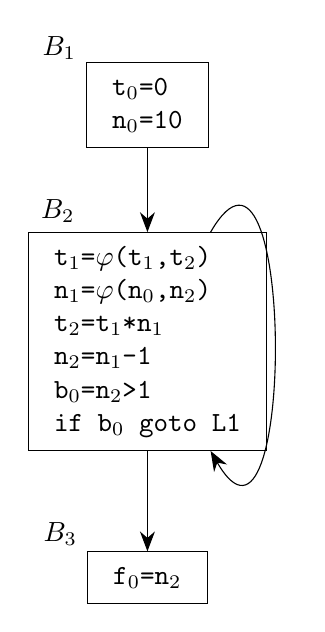
\begin{tikzpicture}
    \node[draw,label={150:{$B_1$}}] (N1) at (0,0) {
        \begin{tabular}{l}
        \verb|t|$_0$\verb|=0|\\
        \verb|n|$_0$\verb|=10|\\
        \end{tabular}};
    \node[draw,label={120:{$B_2$}}] (N2) at (0,-3) {
        \begin{tabular}{l}
            \verb|t|$_1$\verb|=|$\varphi$\verb|(t|$_1$\verb|,t|$_2$\verb|)|\\
            \verb|n|$_1$\verb|=|$\varphi$\verb|(n|$_0$\verb|,n|$_2$\verb|)|\\
            \verb|t|$_2$\verb|=t|$_1$\verb|*n|$_1$\\
            \verb|n|$_2$\verb|=n|$_1$\verb|-1|\\
            \verb|b|$_0$\verb|=n|$_2$\verb|>1|\\
            \verb|if b|$_0$\verb| goto L1|\\
        \end{tabular}
    };
    \node[draw,label={160:{$B_3$}}] (N3) at (0,-6) {
        \begin{tabular}{l}
        \verb|f|$_0$\verb|=n|$_2$
        \end{tabular}
    };
    \path[-{Stealth[scale=1.5]}] (N1) edge (N2);
    \path[-{Stealth[scale=1.5]}] (N2) edge (N3);
    \path[-{Stealth[scale=1.5]}] [out=60,in=300,looseness=2] (N2) edge (N2);
\end{tikzpicture}
\end{document}